\textbf{1.} Khi cường độ điện trường áp vào vẫn chưa đủ mạnh để làm cho chất lỏng phun ra thành
các hạt mang điện thì áp suất tĩnh điện kéo các hạt ra phải nhỏ hơn áp suất do suất căng giữ nó lại:
\begin{equation}
    \frac{1}{2} \varepsilon_0 E^2<\frac{2 \sigma}{R_c}.
    \label{eq:P3_1}
\end{equation}

\textbf{2.} Nếu điện thế \( \phi \) là một hằng số \( (V) \) trên mặt \( \eta = \eta_0 \), và bằng không trên mặt phẳng \( S \), thì toàn bộ nghiệm của \( \phi \) sẽ chỉ phụ thuộc vào \( \eta \). \vspace{1.5mm}

\textbf{3.} Từ phương trình (\ref{i}) và ý \textbf{2} ta có:
\begin{equation}
    (1- \eta ^2) \frac{\mathrm{d} \phi}{\mathrm{d} \eta}=\text{cte} \Rightarrow \mathrm{d} \phi= \text{cte}\frac{ \mathrm{d} \eta}{1- \eta ^2}.
    \label{eq:P3_2}
\end{equation}
Tích phân phương trình (\ref{eq:P3_2}) với $\phi$ chạy từ 0 đến $V$, $\eta$ chạy từ 0 đến $\eta_0$, ta tính được:
\begin{equation}
    \text{cte}=\frac{V}{\tanh^{-1}{\eta_0}}.
    \label{eq:P3_3}
\end{equation}
Khi đó dễ dàng suy ra:
\begin{equation}
    \phi=V \frac{\tanh^{-1}{\eta}}{\tanh^{-1}{\eta_0}}.
    \label{eq:P3_4}
\end{equation}

\textbf{4.} Gọi \( R^2 = x^2 + y^2 \) là bán kính trụ (cylindrical radius).  
Từ biểu thức \( \eta = \dfrac{r_1 - r_2}{a} \), ta thu được mối quan hệ giữa \( z \) và \( R \) đối với mặt hyperboloid có \( \eta \) không đổi:
\begin{equation}
a \eta = \sqrt{R^2 + \left(z + \frac{a}{2} \right)^2} - \sqrt{R^2 + \left(z - \frac{a}{2} \right)^2}.
\label{eq:P3_5}
\end{equation}
Với \( z > 0 \), phương trình (\ref{eq:P3_5}) có thể được rút gọn thành:
\begin{equation}
z = \eta \sqrt{ \frac{a^2}{4} + \frac{R^2}{1 - \eta^2} }.
\label{eq:P3_6}
\end{equation}


Khoảng cách từ đỉnh chất lỏng đến mặt phẳng nối đất là
$z(R = 0, \eta = \eta_0)=d  = \dfrac{a}{2} \eta_0$. Từ phương trình (\ref{ii}), bán kính cong $R_c$ tại đỉnh là:
\begin{equation}
    R_c=a \frac{1-\eta^2}{2 \eta}.
\end{equation}
Do đó, nếu biết \( R_c \) và \( d \), ta có thể xác định các tham số \( a \) và \( \eta_0 \):
\begin{equation}
a = 2d \sqrt{1 + \frac{R_c}{d}} \quad \text{và} \quad \eta_0 = \left(1 + \frac{R_c}{d} \right)^{-1/2}.
\end{equation}
Điện trường tại đỉnh chất lỏng là:
\begin{equation}
E_{\text{đỉnh}} = -\left. \frac{\partial \phi}{\partial z} \right|_{\text{đỉnh}} 
= -\left. \frac{\partial \phi}{\partial \eta} \cdot \frac{\partial \eta}{\partial z} \right|_{\text{đỉnh}}.
\end{equation}
Tại đỉnh ta có \( R = 0 \) và \( \eta = \eta_0 \), nên từ phương trình (\ref{eq:P3_6}):
\begin{equation}
\left. \frac{\partial \eta}{\partial z} \right|_{\text{đỉnh}} = \frac{2}{a}.
\end{equation}
Kết hợp với phương trình (\ref{eq:P3_4}), ta có:
\begin{equation}
E_{\text{đỉnh}} = -\frac{2V / a}{(1 - \eta_0^2) \tanh^{-1} \eta_0}.
\end{equation}
Biểu thức này có thể được viết lại theo \( R_c \) và \( d \), trong trường hợp \( R_c \ll d \), như sau:
\begin{equation}
E_{\text{đỉnh}} = -\frac{2V / R_c}{\ln\left(4d / R_c\right)}.
\label{eq:P3_12}
\end{equation}
Giờ đây, để chất lỏng có thể bị kéo ra thì điều kiện cần là:
\begin{equation}
\frac{1}{2} \varepsilon_0 E_{\text{đỉnh}}^2 \geq \frac{2\sigma}{R_c}.
\label{eq:P3_13}
\end{equation}
Thay phương trình (\ref{eq:P3_12}) vào (\ref{eq:P3_13}), ta được giá trị của $V_{\mathrm{start}}$ là:
\begin{equation}
V_{\mathrm{start}} = \sqrt{ \frac{\sigma R_c}{\varepsilon_0} } \ln\left( \frac{4d}{R_c} \right).
\end{equation}

\textbf{5.} Ý tưởng cơ bản là lực "kéo bề mặt'' trên một đơn vị diện tích 
$\dfrac{\varepsilon_{0}E^{2}}{2}$ do điện trường gây ra phải được cân bằng ở mọi nơi trên bề mặt hình nón với lực kéo của sức căng bề mặt. Lực này tính theo đơn vị diện tích được cho bởi
$\sigma \left( R_{c1}^{-1} + R_{c2}^{-1} \right)$,
trong đó $R_{c1}$ và $R_{c2}$ là hai độ cong chính của bề mặt.

Đối với hình nón, $1 / R_{c1}$ bằng 0 dọc theo đường sinh, trong khi độ cong $1 / R_{c2}$ của mặt cắt pháp tuyến là hình chiếu của độ cong của mặt cắt tròn đi qua cùng điểm đó:
\begin{equation}
\frac{1}{R_c} = \frac{\cos \theta_T}{R} = \frac{\cos \theta_T}{r \sin \theta_T} = \frac{\cot \theta_T}{r}.
\end{equation}
\begin{center}


\tikzset{every picture/.style={line width=0.75pt}} %set default line width to 0.75pt        

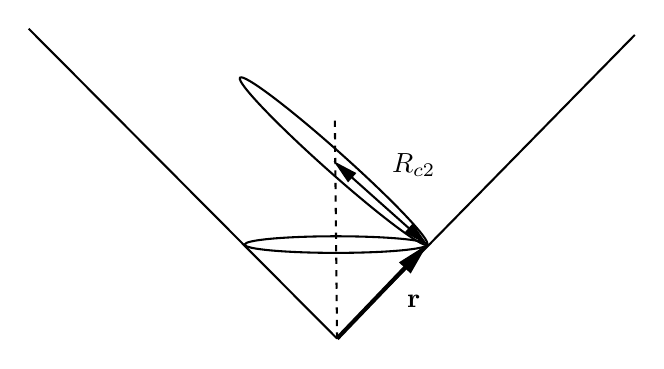
\begin{tikzpicture}[x=0.75pt,y=0.75pt,yscale=-1,xscale=1]
%uncomment if require: \path (0,300); %set diagram left start at 0, and has height of 300

%Straight Lines [id:da477806425534132] 
\draw    (141.43,30.71) -- (290,180) ;
%Straight Lines [id:da3193423659756527] 
\draw    (433.43,33.71) -- (290,180) ;
%Straight Lines [id:da25585832494924077] 
\draw  [dash pattern={on 2.25pt off 2.25pt on 2.25pt off 2.25pt}]  (288.93,75) -- (290,180) ;
%Straight Lines [id:da4333818805346543] 
\draw [line width=1.5]    (290,180) -- (330.66,137.6) ;
\draw [shift={(333.43,134.71)}, rotate = 133.8] [fill={rgb, 255:red, 0; green, 0; blue, 0 }  ][line width=0.08]  [draw opacity=0] (15.6,-3.9) -- (0,0) -- (15.6,3.9) -- cycle    ;
%Shape: Ellipse [id:dp8987360260206204] 
\draw   (243.23,54.3) .. controls (245.07,52.23) and (266.76,68.56) .. (291.66,90.77) .. controls (316.57,112.97) and (335.27,132.65) .. (333.43,134.71) .. controls (331.59,136.78) and (309.91,120.45) .. (285,98.24) .. controls (260.09,76.04) and (241.39,56.36) .. (243.23,54.3) -- cycle ;
%Shape: Ellipse [id:dp9630900939952156] 
\draw   (245.43,134.71) .. controls (245.43,132.5) and (265.13,130.71) .. (289.43,130.71) .. controls (313.73,130.71) and (333.43,132.5) .. (333.43,134.71) .. controls (333.43,136.92) and (313.73,138.71) .. (289.43,138.71) .. controls (265.13,138.71) and (245.43,136.92) .. (245.43,134.71) -- cycle ;
%Straight Lines [id:da46867561246502043] 
\draw    (289.82,95.84) -- (331.94,133.38) ;
\draw [shift={(333.43,134.71)}, rotate = 221.72] [fill={rgb, 255:red, 0; green, 0; blue, 0 }  ][line width=0.08]  [draw opacity=0] (12,-3) -- (0,0) -- (12,3) -- cycle    ;
\draw [shift={(288.33,94.51)}, rotate = 41.72] [fill={rgb, 255:red, 0; green, 0; blue, 0 }  ][line width=0.08]  [draw opacity=0] (12,-3) -- (0,0) -- (12,3) -- cycle    ;

% Text Node
\draw (322.21,157.76) node [anchor=north west][inner sep=0.75pt]    {$\mathbf{r}$};
% Text Node
\draw (315,89.4) node [anchor=north west][inner sep=0.75pt]    {$R_{c2}$};


\end{tikzpicture}

\end{center}
Điều này dẫn đến:
\begin{equation}
\frac{1}{2} \varepsilon_0 E_n^2 = \frac{\sigma \cot \theta_T}{r} \quad \text{hay} \quad E_n = \sqrt{\frac{2 \sigma \cot \theta_T}{\varepsilon_0 r}}.
\end{equation}

%% Reference %%
\bibliographystyle{plain}
\begin{thebibliography}{}
\bibitem{Electrospray} Massachusetts Institute of Technology. “\textit{Electrospray Propulsion}.” Lecture 20 of 16.522 \textit{Space Propulsion}, Spring 2015, instructors Manuel Martinez-Sanchez and Paulo Lozano. \url{https://ocw.mit.edu/courses/16-522-space-propulsion-spring-2015/6fe2f497158a264687e8f962eac3db35_MIT16_522S15_Lecture20.pdf}
\end{thebibliography}